\section{Refinement}

% Nice but long
\begin{comment} 
The refinement relation aims at formalizing the relation between
abstract and concrete versions of the same component, or between an
abstract component and its implementation.  
In the input-enabled (or pessimistic) setting, refinement is usually
defined as trace containment or simulation
\cite{Milner71}: this ensures that the set of output behaviors of the
implementation is a subset of that of the abstract component.  
However, such definitions are not be appropriate in a
non-input-enabled setting such as our interfaces: they would also
require that the set of legal inputs of the implementation is a
subset of that of the abstract component --- implying that the
implementation can be used in fewer environments than the abstract
component was designed for.
%
For example, if we adopted the classical definition, then the
component $\adder$ of Figure~\ref{fig-counter} would be refined by
a component $\strongadder$ having the same output transition relation, 
but that does not perform subtraction: precisely, with the 
{\em single\/} input guard {\tt [] true -> q1':=1}. 
%
As this example points out, refinement should be defined in a
contravariant fashion: the implementation should accept more inputs,
and produce fewer outputs, than the specification
\cite{luca-ia-01,luca-it-01}. 
\end{comment}

We define refinement as alternating simulation \cite{CONCUR98AHKV}:
roughly, a component $\mq$ refines $\mp$ (written $\mq \refi \mp$) if
$\mq$ can simulate all inputs of $\mp$, and if $\mp$ can simulate all
outputs of $\mq$.
Encoding the relation between the states of two Moore interfaces
$\mp$ and $\mq$ by a predicate $\rrp$, we can state the definition of
refinement as follows. 

\begin{defi}{(Refinement of Moore interfaces)}
\label{def-moore-ref} 
Given two Moore interfaces $\mp$ and $\mq$, 
% let $\avars = \ovars_\mp \setm \ovars_\mq$ be the set of ``private''
% variables of the specification. 
we have that $\mq \refi \mp$ if $\ivars_\mq \subs \ivars_\mp$ and 
$\ivars_\mp \inters (\ovars_\mp \union \ovars_\mq) = \emptyset$, 
and if there is a predicate $\rrp$ on $\vars_\mp \union \vars_\mq$
such that the following formulas are valid: 
%
\begin{eqalignno*}
\label{eq-moore-ref} 
  \iinit_\mp \und \oinit_\mq & \;\;\im \;\;
	\exists (\ovars_\mp \setm \ovars_\mq).
	(\iinit_\mq \und \oinit_\mp \und \rrp) \\
\rrp \und \itrans_\mp \und \otrans_\mq & \;\;\im\;\;
  \exists (\ovars_\mp \setm \ovars_\mq)'. 
	(\itrans_\mq \und \otrans_\mp \und \rrp') \hspace{2em} \qed 
\end{eqalignno*}
\end{defi}

% \noindent
% As an example, let $\adder'$ be the Moore interface obtained from
% $\adder$ by dropping the guarded command {\tt [] true -> q1':=1}, 
% and let $\adder''$ be the interface obtained from
% $\adder'$ by adding the guarded command {\tt q0 -> do':=do}. 
% Then, $\adder \refi \adder' \refi \adder''$, and the converse
% refinements do not hold. 

% \subsection{Implementation considerations} 

\noindent
As for normal simulation, there is a unique largest
refinement relation between any two Moore interfaces. 
% in fact, the union of two refinement relations is again a refinement
% relation. 
% In fact, indicating with 
% $\Psi_\tau(\rrp)$ and $\Psi_\theta(\rrp)$ the two formulas of 
% (\ref{eq-moore-ref}), it easy to see that if both 
% $\Psi_\tau(\rrp_1) \und \Psi_\theta(\rrp_1)$
% and
% $\Psi_\tau(\rrp_2) \und \Psi_\theta(\rrp_2)$, 
% then also 
% $\Psi_\tau(\rrp_1 \oder \rrp_2) \und \Psi_\theta(\rrp_1 \oder \rrp_2)$.
Hence, Definition~\ref{def-moore-ref}
provides an iterative algorithm for deciding refinement: 
let $\rrp_0 = \true$, and for $k \geq 0$, let 
%
\begin{equation} \label{eq-refi-comp} 
  \rrp_{k+1} = \rrp_k \und \forall (\vars_\mp \union \vars_\mq)' . 
  \bigl(\itrans_\mp \und \otrans_\mq \im 
  \exists (\ovars_\mp \setm \ovars_\mq)' . 
  (\itrans_\mq \und \otrans_\mp \und \rrp_k')\bigr).
\end{equation}
% 
Denoting with $\rrp_* = \lim_{k \go \infty} \rrp_k$ the fixpoint
(that again can be computed in a finite number of iterations), 
we have that $\mq \refi \mp$ if and only if (i)~$\ivars_\mq \subs
\ivars_\mp$ and  $\ivars_\mp \inters (\ovars_\mp \union \ovars_\mq) =
\emptyset$, and (ii)~$\iinit_\mp \und \oinit_\mq \;\im\; \exists 
(\ovars_\mp \setm \ovars_\mq) . (\iinit_\mq \und \oinit_\mp \und \rrp)$. 
In order to obtain an efficient implementation, we can again take
advantage for the computation of (\ref{eq-refi-comp}) of list
representations for the transition relations, and apply
image-computation techniques. 

Refinement of bidirectional  interfaces is defined similarly,
except that the refinement relation relates the locations of the two
interfaces, rather than the states. 
The definition is as follows. 

\begin{defi}{(Refinement of bidirectional  interfaces)}
Given two bidirectional  interfaces $\mp$ and $\mq$, $\mq$ refines
$\mp$ ($\mq \refi \mp$) iff there is 
% an alternating  simulation
% $\refi$ of $\mq$ by $\mp$ with $\hat{q}_{\mq} \refi \hat{q}_\mp$. 
% An alternating  simulation of $\mq$ by $\mp$ is 
a binary relation $\refi \subs Q_{\mq} \times Q_\mp$ 
such that $\hat{q}_{\mq} \refi \hat{q}_\mp$, 
and such that for all $q \refi p$ we have 
(i)~$\ivarsf_\mq(q) \subs \ivarsf_\mp(q)$, 
(ii)~$\ovarsf_{\mq}(q) \supseteq \ovarsf_\mp(p)$, 
(iii)~$\phi^i_{\mp}(p) \im \phi^i_\mq(q)$, 
(iv)~$\phi^o_\mq(q) \im \phi^o_\mp(p)$, 
(v)~for all $s \in \states[\ivarsf_\mp(p)]$ 
and all $t \in \states[\ovarsf_\mq(q)]$, 
if $s \sat \trel_\mp(p,p')$ and $t \sat \trel_\mq(q,q')$, 
then $q' \refi p'$. \qed 
\end{defi}

\noindent
We can check whether $\mq \refi \mp$ by adapting the classical
iterative refinement check \cite{Milner71}. 
We start with the total relation $\refi_0 = Q_\mq \times Q_\mp$, and
for $k \geq 0$, we let $\refi_{k+1}$ be the subset of $\refi_k$ such
that conditions~(i)--(v) hold, with $\refi_k$ in place of $\refi$ in
condition~(v). 
Once we reach $m \geq 0$ such that $\refi_{m+1} = \refi_m$, we have
that $\mq \refi \mp$ iff $\hat{q}_\mq \refi \hat{p}_\mq$. 
Since bidirectional interfaces are deterministic we can reduce
the refinement checking problem to graph reachability on the product
interface and hence $\mq \refi \mp$ can be decided in $O(|Q_\mq| \times
|Q_\mp|)$ time.

\begin{comment} 
%
% WARNING: old notation
%
\mynote{I cut out the algorithm here} 
\begin{algorithm}[ht]
\caption{Refinement Check for Stateful Bidirectional  Interfaces} \label{algo2}
\begin{algorithmic}[1]
\REQUIRE two stateful bidirectional  interfaces 
$F = (P_F,Q_F,\hat{q}_F,o_F,o^+_F,\phi_F,\psi_F,\delta_F)$ and
$F' = (P_{F'},Q_{F'},\hat{q}_{F'},o_{F'},o^+_{F'},\phi_{F'},\psi_{F'},\delta_{F'})$
\STATE Let $Prod_{F,F'} = F \circledast F' =$ a \emph{directed graph} 
$G(V_{Prod},E_{Prod})$ where 
$V_{Prod} = Q_F \times Q_{F'}$ and $E_{Prod} \subs V_{Prod} \times V_{Prod}$
such that $e = (v_1,v_2) \in E_{Prod}$ iff $v_1 = (q_1,q'_1)$, $v_2 = (q_2,q'_2)$
and $\exists$ valuations $i \in [P_F - o^+_F(q_1)]$, $o' \in [o_{F'}(q'_1]$ such that 
$\phi_F(q_1) @ i$ and $\psi_{F'}(q'_1) @ o'$ and $q_2 = \delta_F(q_1,i \uplus o')$
and $q'_2 = \delta_{F'}(q'_1,i \uplus o')$.
\STATE Let a state $v = (q,q')$ be an {\em error} state iff 
$(o_{F'}(q') \nsupseteq o_F(q)) \lor (o^+_{F'}(q') \nsubseteq o^+_F(q)) 
\lor (P_{F'} - o^+_{F'}(q') \nsubseteq P_F - o^+_F(q)) \lor 
(\phi_F(q) \nRightarrow \phi_{F'}(q')) \lor 
(\psi_{F'}(q') \nRightarrow \psi_F(q))$.
\IF {any error state is reachable from $(\hat{q}_F,\hat{q}_{F'})$ in 
$G(V_{Prod},E_{Prod})$}
\STATE $F'$ does not refine $F$
\ELSE
\STATE $F'$ refines $F$
\ENDIF
\end{algorithmic}
\end{algorithm}
\end{comment} 

\begin{examp}{(Token Ring)}
The IEEE 802.5 (Token Ring) is a widely used deterministic 
LAN protocol. Figure~\ref{tokenringstate} shows an interface modeling
a node that initially does not have the token. 
The same diagram with $T$ as initial state would 
represent a node that initially has the token. 
We call these two interfaces $NT$ and $T$, respectively.
The token ring components are connected in a cyclic network; each pair
of adjacent nodes communicate by $req$ and $gnt$ signals
(Figure~\ref{tokenringstr}). 
The $req$ signal flows clockwise, and is used to request the token; 
the signal $give$ flows counterclockwise, and is used to grant the token.
%
% As long
% as its $req$ input is de-asserted, it continues to hold the token. 
% When the token is requested, it goes into state $G$. %, where it may or may not 
% give the token to the requesting node immediately. When it decides to 
% give up the token, it asserts its $give$ output, sending the requesting 
% node into state $RR$ and itself going into state $RG$. When the 
% requesting node has got the token, it de-asserts its $req$ output, going 
% into state $T$, and this makes the other go into state $NT$, from which
% the sequence continues as before. The states $RG$ and $RR$ % are of
% technical importance only, to ensure that the token is not lost in transit.
% One would expect this protocol to fail if more than one node has the token 
% simultaneously. We verify this using interface compatibility checking.
% One would expect the protocol to work independent of the number of nodes
% in the network. We verify this using interface refinement.
%
The protocol fails if more than one node has the token simultaneously:
indeed, we can verify that two $T$ interfaces are not compatible,
while an $NT$ interface is compatible with a $T$ interface.  
Moreover, the protocol works for any number of participating nodes. 
To verify this, we check two refinements: 
first, an open-ring configuration consisting entirely of $NT$ nodes is a
refinement of the configuration consisting in just one $NT$ node; 
second, an open-ring configuration with any number of $NT$ nodes and
one $T$ node is a refinement of a configuration consisting in a single
$T$ node.   
Our implementation is able to perform the above compatibility and
refinement checks in a fraction of a second. \qed 
\end{examp}

% \begin{figure}
% \centering
% \subfigure[Token Ring NT interface]{\label{tokenringstate}
% 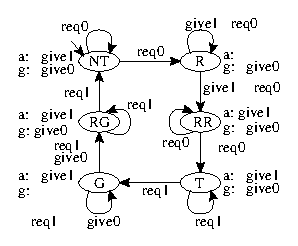
\includegraphics[scale=0.20]{tokenringstate.pstex}}
% \hspace*{2em}
% \subfigure[Token Ring network]{\label{tokenringstr}
% 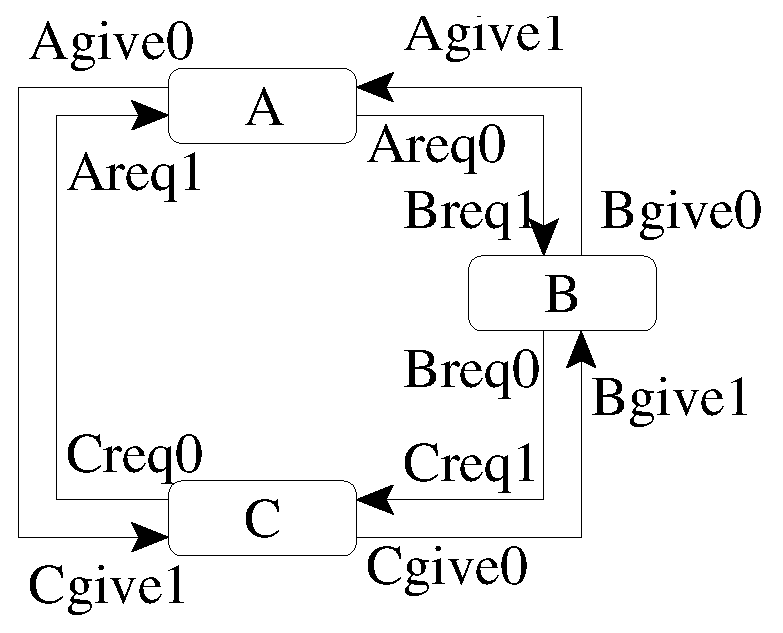
\includegraphics[scale=0.20]{tokenringstr.pstex}}
% \caption{Token ring protocol.} 
% \end{figure}

% The composition of two $T$ interfaces is found to be null. Thus our tool 
% verifies that two $T$ nodes are incompatible, as expected.
% It verifies that a network configuration with $1$ $T$ node and any number 
% of $NT$ nodes is a refinement of a network configuration with just 
% $1$ $T$ node, as expected.  
% Similarly a network configuration with any number of $NT$ nodes and no
% $T$ nodes is verified to be a refinement of a network configuration with 
% just one $NT$ node. 
% A network configuration with $k$ $NT$ nodes and no $T$ nodes is found 
% to be a refinement of a configuration with $n \leq k$ $NT$ nodes and 
% no $T$ nodes.
% This confirms the independence of the token ring protocol of the number
% of participating nodes. \qed

\noindent
The notion of refinement, in addition to implementation, captures also
substitutivity: if $\mq$ refines $\mp$, and $\mp$ is compatible with
the remainder $\mr$ of the design, then $\mr$ is also compatible with
$\mq$. 

\begin{theo}{(Substitutivity of refinement)}
Consider three bidirectional Moore or  bidirectional interfaces
$\mp, \mq, \mr$, such that $\mp\compat\mr$, and $\mq \refi \mp$. 
If $(\ovars_\mq \inters \ivars_\mr) \subs (\ovars_\mp \inters \ivars_\mr)$,
then $\mq\compat\mr$ and $(\mq \| \mr) \refi (\mp \| \mr)$. 
\end{theo}

\noindent
The  result has a proviso: all the variables that are output by $\mq$
and input by $\mr$ should also be output by $\mp$. 
If this were not the case, it would be possible for the additional
outputs of $\mq$ to violate the input assumptions of $\mr$.

